
\documentclass{article}
\usepackage{amsmath}
\usepackage[utf8]{inputenc}
\usepackage{ctex}
\usepackage{indentfirst}

\usepackage{graphicx}

\usepackage{listings}
\usepackage{color}
\usepackage[hidelinks]{hyperref}


\lstset{
    language=Python, % 设置语言
    basicstyle=\ttfamily, % 基本字体样式
    keywordstyle=\color{blue}, % 关键词的颜色
    commentstyle=\color{green}, % 注释的颜色
    stringstyle=\color{red}, % 字符串的颜色
    showstringspaces=false, % 不显示字符串间隙
    numbers=left, % 显示行号
    numberstyle=\tiny\color{gray}, % 行号样式
    breaklines=true, % 自动换行
    frame=single % 给代码框加一个边框
}


\setlength{\parindent}{2em}

\begin{document}

\begin{center}
    \Large \textbf{Lab2 实验报告}\\
    \vspace{1em}
    姓名:陈翎玺~~学号:523030910039~~班级:电院2302
\end{center}

\section{实验概览}
    本次实验主要学习了图像边缘的提取和Canny算法的实现。


    图像的大部分信息都存在于图像的边缘中,主要表现为图像局部特征的不连续性,
    即图像中灰度变化比较剧烈的地方。
    因此定义图象的边缘为图象局部区域亮度变化显著的部分,
    该区域的灰度剖面一般可以看作是一个阶跃,
    即灰度值在很小的区域内急剧的变化。


    Canny算法是一种经典的边缘检测算法,由John Canny在1986年提出,
    主要用于图像处理中的边缘提取。
    它的设计目标是最大限度地减少噪声的干扰,
    同时保持边缘的精确性。
    广泛用于目标检测、图像分割、物体识别等领域,是计算机视觉中的重要工具。

    Canny算法的优点包括:
\begin{enumerate}
\item 抗噪性强:高斯滤波减少了噪声的干扰。
\item 检测精确:通过梯度计算和非极大值抑制,确保边缘精度高。
\item 双阈值处理:增强了边缘检测的灵活性。
\end{enumerate}

    Canny算法的主要步骤包括灰度化,高斯滤波,梯度计算,非极大值抑制,
    双阈值处理和边缘连接。其具体步骤将在\ref{section2}中展开。

\section{练习题的解决思路}\label{section2}
\subsection{灰度化}

    通常摄像机获取的是彩色图像,而检测的首要步骤是进行灰度化,
    以RGB格式彩图为例,一般的灰度化方法有两种:

    方法一:
    \[Gary = (R + G + B) / 3\]

\newpage

    方法二:
    \[Gary = 0.299R + 0.587G + 0.114B\]
\begin{center}
(参数考虑人眼的生理特点)
\end{center}

    考虑本题已给出图片,使用opencv的imread(..., cv2.IMREAD\_GRAYSCALE)
    直接读取灰度图即可。

\subsection{高斯滤波}
    为了降低图像中的噪声,首先对图像进行高斯滤波。
    通过卷积操作平滑图像,以减少后续边缘检测时的误检。

    图像高斯滤波的实现可以用两个一维高斯核分别两次加权实现,
    也可以通过一个二维高斯核一次卷积实现
    离散化的一维高斯函数与二维高斯函数如下:

    \[K = \frac{1}{\sqrt{2\pi}\sigma}e^{-\frac{x^2}{2\sigma^2}}\]
\begin{center}
    离散一维高斯函数
\end{center}

    \[K = \frac{1}{2\pi\sigma^2}e^{-\frac{x^2 + y^2}{2\sigma^2}}\]

\begin{center}
    离散二维高斯函数
\end{center}

    具体而言,高斯滤波器核的生成方程式由下式给出:
    \[H_{ij} = \frac{1}{2\pi\sigma^2}\exp(-\frac{(i - (k + 1))^2 + (j - (k + 1)^2)}{2\sigma^2}); 1\leq i, j \leq (2k + 1)\]

    本次实验取\(k = 1, \sigma = 1.4\),得到对应的高斯滤波器核(归一化后)的结果为

\[
H = \begin{bmatrix}
0.0924 & 0.1192 & 0.0924 \\
0.1192 & 0.1538 & 0.1192 \\
0.0924 & 0.1192 & 0.0924
\end{bmatrix}
\]

若图像中一个3x3的窗口为A,要滤波的像素点为e,则经过高斯滤波之后,像素点e的亮度值为:

\[
e = H * A = \begin{bmatrix}
H_{11} & H_{12} & H_{13} \\
H_{21} & H_{22} & H_{23} \\
H_{22} & H_{32} & H_{33}
\end{bmatrix}
*
\begin{bmatrix}
a & b & c \\
d & e & f \\
g & h & i
\end{bmatrix}
=
sum\left(\begin{bmatrix}
a\times H_{11} & b\times H_{12} & c\times H_{13} \\
d\times H_{21} & e\times H_{22} & f\times H_{23} \\
g\times H_{22} & h\times H_{32} & i\times H_{33}
\end{bmatrix}\right)
\]

    其中*为卷积符号,sum表示矩阵中所有元素相加求和

\subsection{梯度计算}\label{operator}

    关于图像灰度值得梯度可使用一阶有限差分来进行近似,
    这样就可以得图像在x和y方向上偏导数的两个矩阵。
    常用的梯度算子有如下几种(本次实验使用Sobel算子):

\subsubsection{Roberts算子}

\[
s_x =
\begin{bmatrix}-1 & 0 \\ 0 & 1
\end{bmatrix}
\quad
s_y =
\begin{bmatrix}0 & -1 \\ 1 & 0
\end{bmatrix}
\]

定义窗口\[A = \begin{bmatrix}f_{i,j} & f_{i, j + 1} \\ f_{i + 1, j} & f_{i + 1, j + 1}
\end{bmatrix}\]

对应的梯度矩阵为
\[
G_{x, i,j} = sum\left( s_x * A \right)
\]

\[G_{y, i,j} = sum\left( s_y * A \right)
\]

\[G_{i,j} = \lvert  G_{x, i,j}\rvert + \lvert G_{y, i,j}\rvert \]

\subsubsection{Sobel算子}\label{sobel}

\[
s_x =
\begin{bmatrix}-1 & 0 & 1\\ -2 & 0 & 2 \\ -1 & 0 & 1
\end{bmatrix}
\quad
s_y =
\begin{bmatrix}1 & 2 & 1 \\ 0 & 0 & 0 \\ -1 & -2 & 1
\end{bmatrix}
\]

定义窗口\[A = \begin{bmatrix}f_{i - 1, j - 1} & f_{i - 1, j} & f_{i - 1, j + 1} \\f_{i, j - 1} & f_{i,j} & f_{i, j + 1} \\ f_{i + 1, j - 1} & f_{i + 1, j} & f_{i + 1, j + 1}
\end{bmatrix}\]

对应的梯度矩阵为
\[
G_{x, i,j} = sum\left( s_x * A \right)
\]

\[G_{y, i,j} = sum\left( s_y * A \right)
\]

\[G_{i,j} = \sqrt{G_{x, i,j}^2 + G_{y, i,j}^2}\]

\subsubsection{Prewitt算子}

\[
s_x =
\begin{bmatrix}-1 & 0 & 1\\ -1 & 0 & 1 \\ -1 & 0 & 1
\end{bmatrix}
\quad
s_y =
\begin{bmatrix}1 & 1 & 1 \\ 0 & 0 & 0 \\ -1 & -1 & 1
\end{bmatrix}
\]

定义窗口
\[A = \begin{bmatrix}f_{i - 1, j - 1} & f_{i - 1, j} & f_{i - 1, j + 1} \\f_{i, j - 1} & f_{i,j} & f_{i, j + 1} \\ f_{i + 1, j - 1} & f_{i + 1, j} & f_{i + 1, j + 1}
\end{bmatrix}\]

对应的梯度矩阵为
\[
G_{x, i,j} = sum\left( s_x * A \right)
\]

\[G_{y, i,j} = sum\left( s_y * A \right)
\]

\[G_{i,j} = \sqrt{G_{x, i,j}^2 + G_{y, i,j}^2}\]

\subsubsection{Canny算子}

\[
s_x =
\begin{bmatrix}-1 & 1 \\ -1 & 1
\end{bmatrix}
\quad
s_y =
\begin{bmatrix}1 & 1 \\ -1 & -1
\end{bmatrix}
\]

定义窗口\[A = \begin{bmatrix}f_{i,j} & f_{i, j + 1} \\ f_{i + 1, j} & f_{i + 1, j + 1}
\end{bmatrix}\]

对应的梯度矩阵为
\[
G_{x, i,j} = sum\left( s_x * A \right) / 2
\]

\[G_{y, i,j} = sum\left( s_y * A \right) / 2
\]

\[G_{i,j} = \sqrt{G_{x, i,j}^2 + G_{y, i,j}^2}
\]

\subsection{非极大值抑制}

    图像梯度幅值矩阵中的元素值越大,说明图像中该点的梯度值越大。
    在Canny算法中,非极大值抑制是进行边缘检测的重要步骤,
    是指寻找像素点局部最大值,将非极大值点所对应的灰度值置为0,
    从而可以剔除掉一大部分非边缘点。

    如图:
\begin{figure}[h]
    \centering
    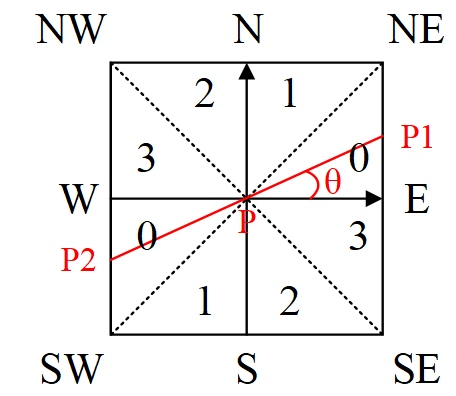
\includegraphics[width=0.4\textwidth]{./report/img}
    \caption{非极大值抑制示意图}
\end{figure}

    由\ref{sobel}得到的\(G_{x, i,j}\)(向右)和\(G_{y, i,j}\)(向上)梯度,
    可以计算得该点的梯度方向。
    红色线条方向为C点的梯度方向,C点局部的最大值则分布在这条线上。

    由于像素是离散存储的,梯度方向不一定恰好命中邻域中的点(如本图中的P1,P2)。
    为了得到对应点的像素值,我们可以通过插值的方法计算P1,P2的值。

    对于图中这种情况,
    \[\lvert G_{y, i,j} \rvert \leq \lvert G_{x, i,j}\rvert, G_{x, i,j}\times G_{y, i,j} > 0\]

    计算方法如下所示如下所示:
\[
    k = G_{y, i,j} / G_{x, i,j}
\]
\[
    P1 = NE \times k + E \times (1 - k)
\]
\[
    P2 = SW \times k + E \times (1 - k)
\]

    其中,\(NW = G_{i - 1, j - 1}, N = G_{i - 1, j}, \ldots, SE = G_{i + 1, j + 1}\)
    如果\(G_{i, j} \geq P1\)且\(G_{i, j} \geq P2\),那么说明点\(\left( i, j \right)\)
    是梯度极大值点,保留。否则丢弃它。

    对于其他情况,同理计算并插值即可,具体方法可见代码。

\subsection{双阈值处理和边缘连接}

    Canny算法中减少假边缘数量的方法是采用双阈值法。
    选择两个阈值,根据高阈值得到一个边缘图像,
    这样一个图像含有很少的假边缘,但是由于阈值较高,
    产生的图像边缘可能不闭合,为解决此问题采用了另外一个低阈值。
    对非极大值抑制图像作用两个阈值th1和th2,
    两者关系th1=0.4th2

    在高阈值图像中把边缘链接成轮廓,
    当到达轮廓的端点时,该算法会在断点邻域点中寻找满足低阈值的点,
    再根据此点收集新的边缘,直到整个图像边缘闭合。

\section{代码运行结果和结果分析}

\subsection{灰度化和高斯模糊}
\newpage

\begin{figure}[h]
    \centering
    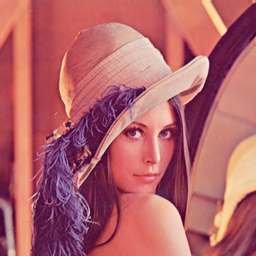
\includegraphics[width=0.25\textwidth]{./dataset/1}
    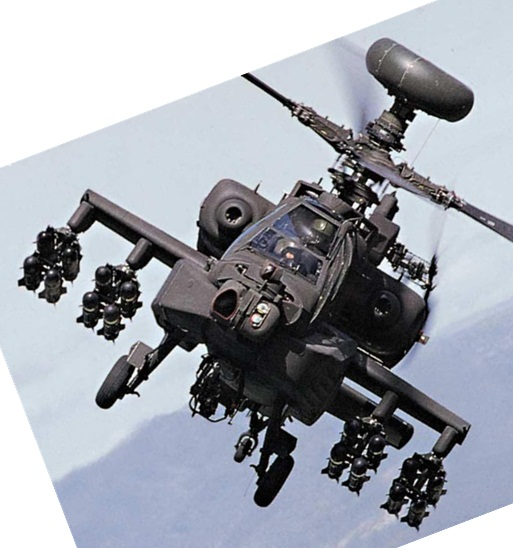
\includegraphics[width=0.25\textwidth]{./dataset/2}
    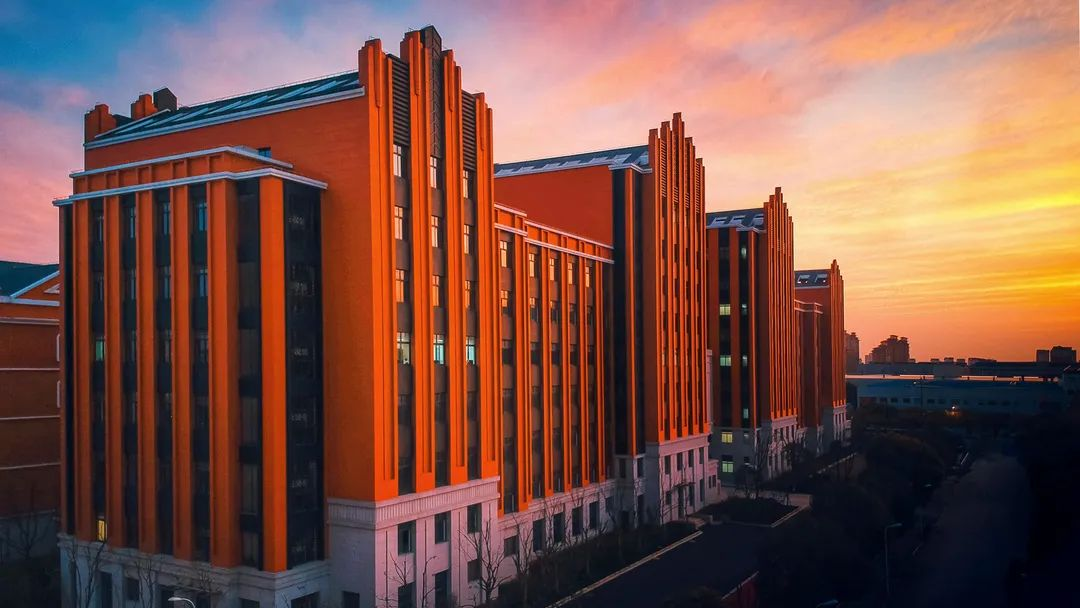
\includegraphics[width=0.25\textwidth]{./dataset/3}
    \caption{原始图}
\end{figure}

\begin{figure}[h]
    \centering
    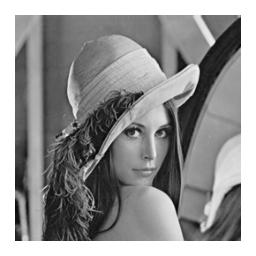
\includegraphics[width=0.25\textwidth]{./grey_image/1}
    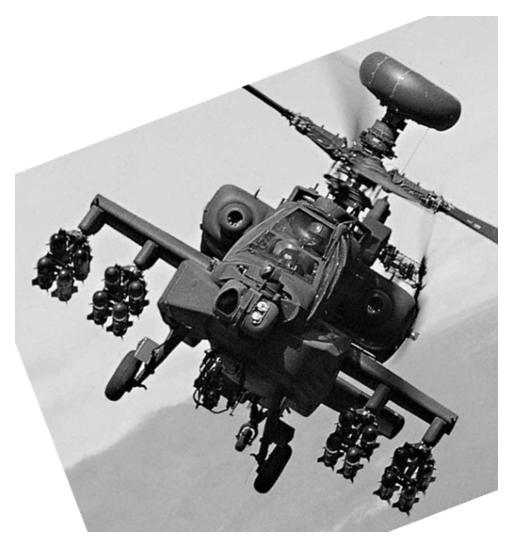
\includegraphics[width=0.25\textwidth]{./grey_image/2}
    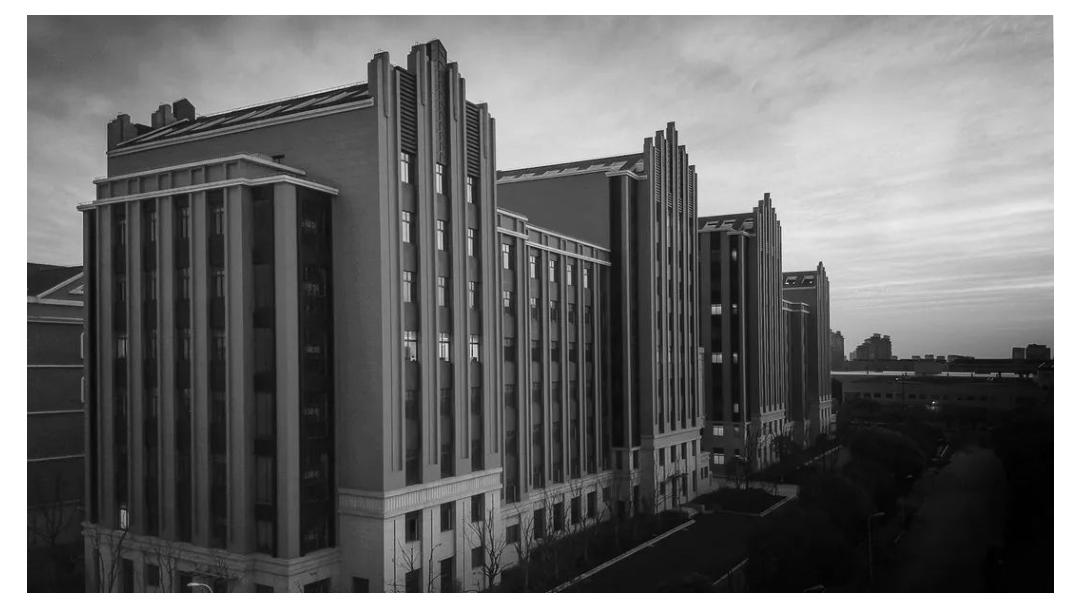
\includegraphics[width=0.25\textwidth]{./grey_image/3}
    \caption{灰度图}\label{figure3}
\end{figure}

\begin{figure}[h]
    \centering
    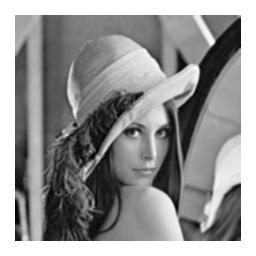
\includegraphics[width=0.25\textwidth]{./gauss_blur/1}
    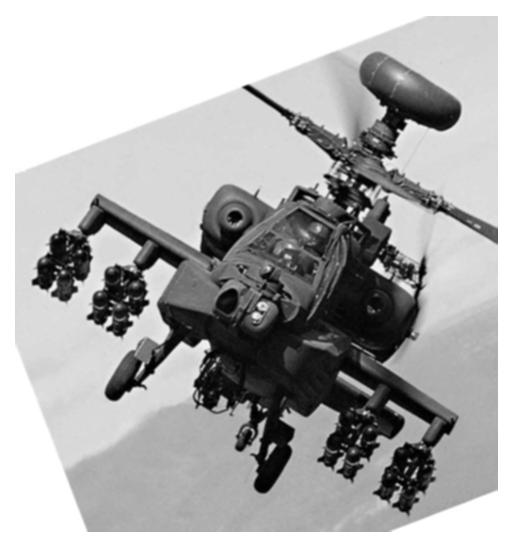
\includegraphics[width=0.25\textwidth]{./gauss_blur/2}
    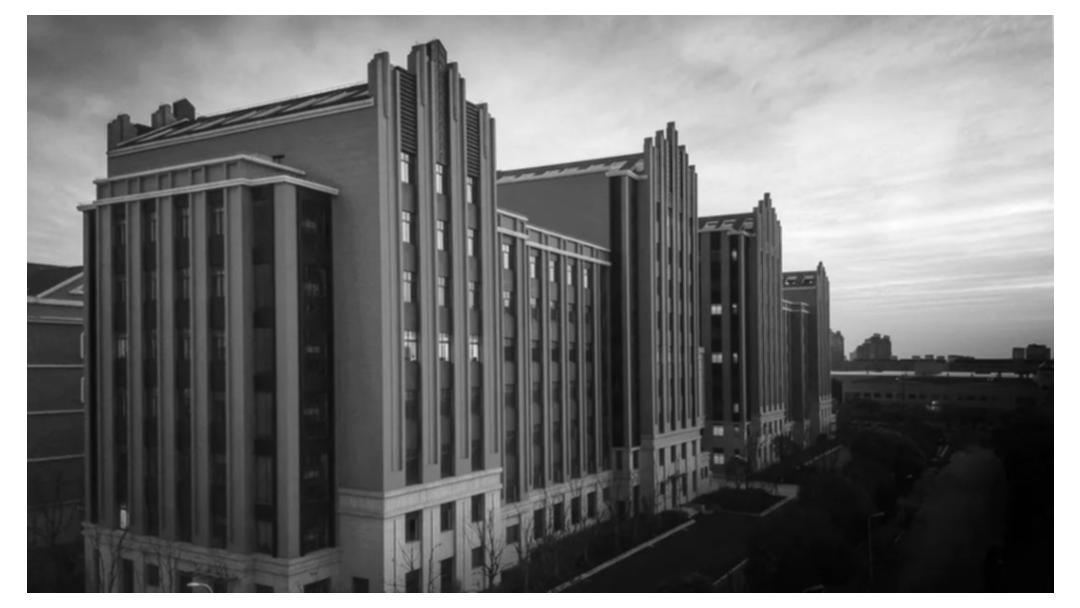
\includegraphics[width=0.25\textwidth]{./gauss_blur/3}
    \caption{高斯模糊}\label{figure4}
\end{figure}

    由图\ref{figure3}和图\ref{figure4}的对比可以看出,
    高斯模糊滤去了一部分高频细节,但同时模糊了噪声,更利于边缘提取,减少假边缘。
    如左图的草帽的纹理,中图直升机螺旋桨的边缘平滑等。

\subsection{梯度可视化和非极大值抑制}
\newpage

\begin{figure}[h]
    \centering
    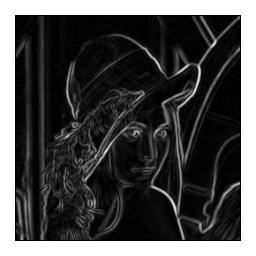
\includegraphics[width=0.25\textwidth]{./sobel_gradmap/1}
    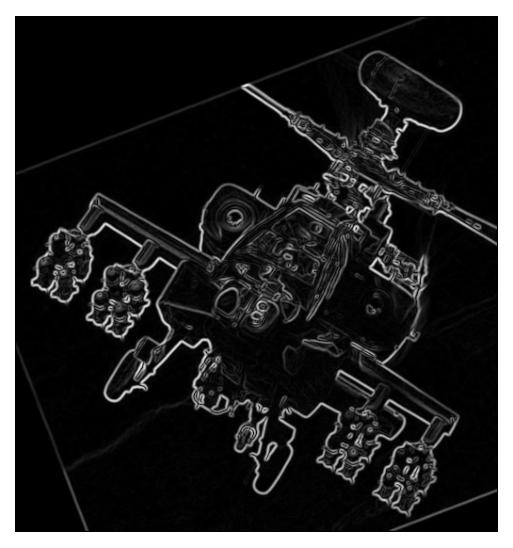
\includegraphics[width=0.25\textwidth]{./sobel_gradmap/2}
    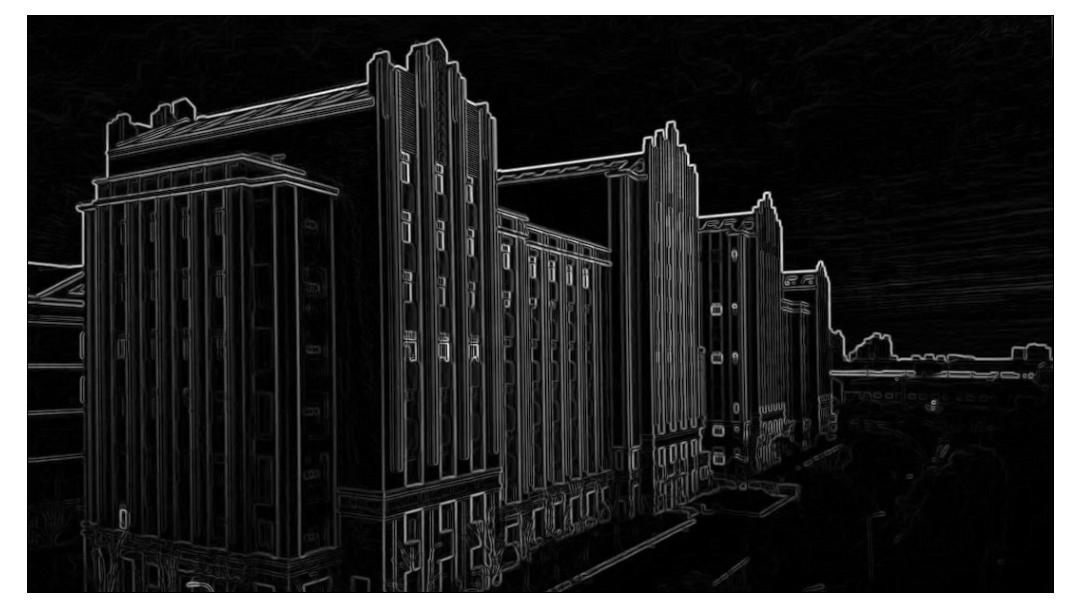
\includegraphics[width=0.25\textwidth]{./sobel_gradmap/3}
    \caption{Sobel算子的梯度}
\end{figure}

\begin{figure}[h]
    \centering
    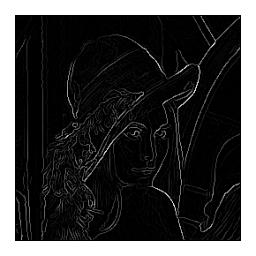
\includegraphics[width=0.25\textwidth]{./filter_notmax/1}
    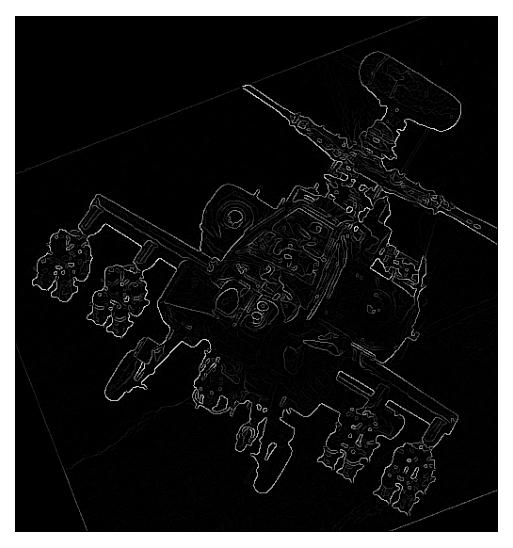
\includegraphics[width=0.25\textwidth]{./filter_notmax/2}
    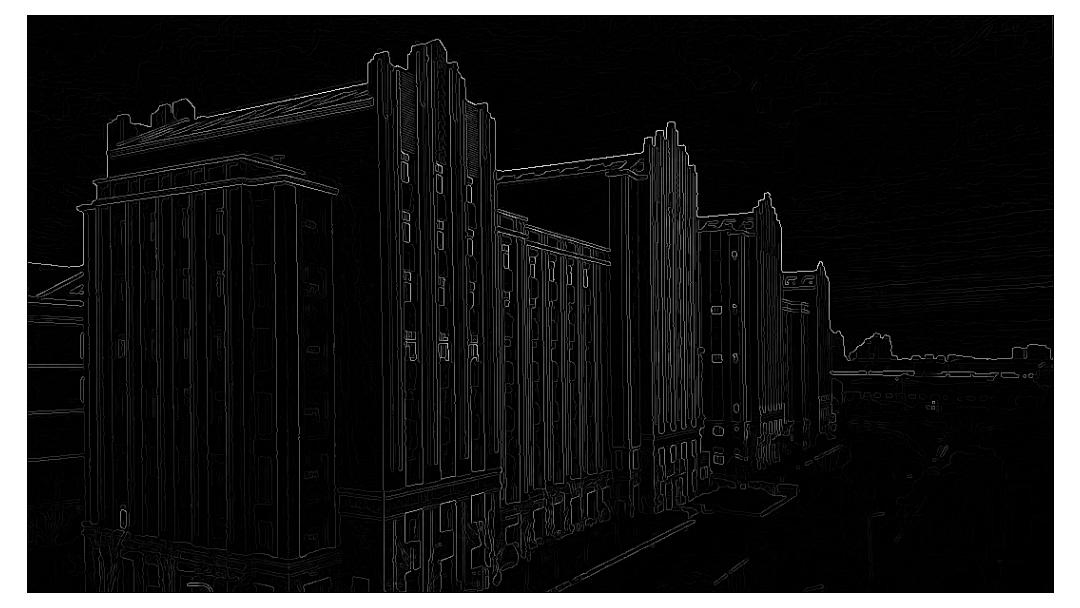
\includegraphics[width=0.25\textwidth]{./filter_notmax/3}
    \caption{非极大值抑制结果}
\end{figure}

    可以看到,经过非极大值抑制,图片的边缘明显变细,精度变好。
    
\subsection{双阈值检测和连接边缘}

\begin{figure}[h]
    \centering
    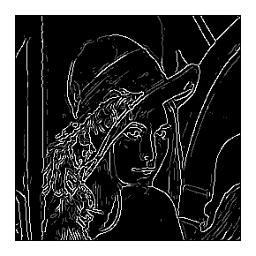
\includegraphics[width=0.25\textwidth]{./classify_100_40/1}
    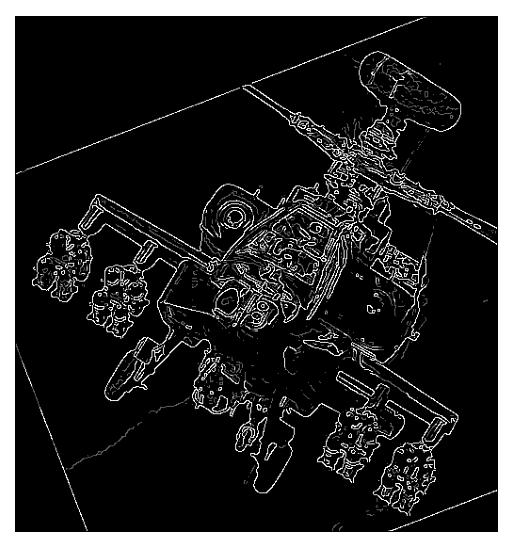
\includegraphics[width=0.25\textwidth]{./classify_100_40/2}
    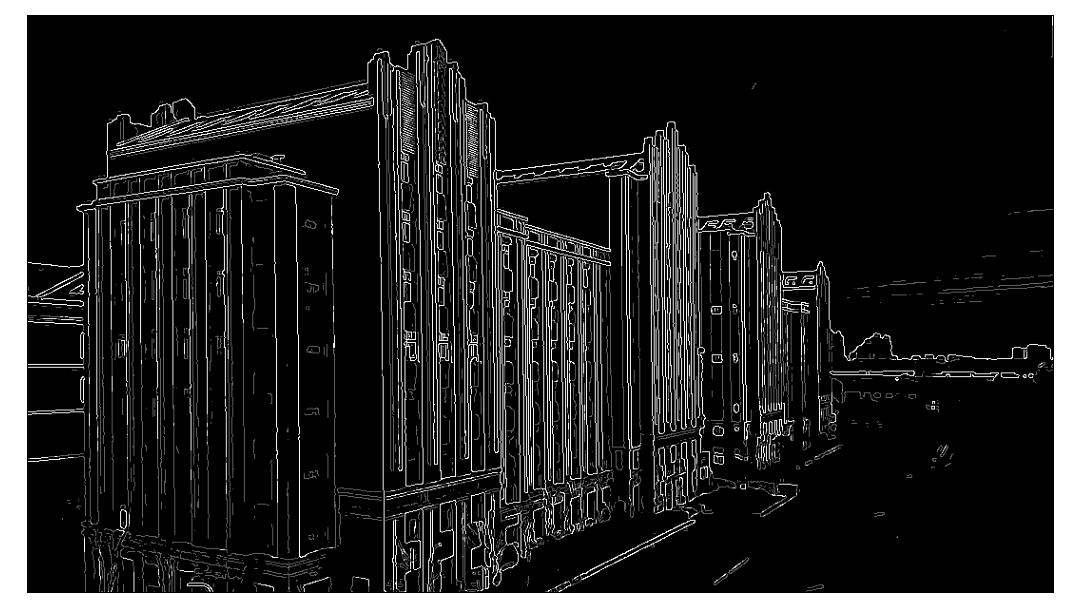
\includegraphics[width=0.25\textwidth]{./classify_100_40/3}
    \caption{双阈值检测结果}
\end{figure}

    这里设置高阈值为100,低阈值为40。
    高低阈值分别对应亮暗像素点,可以发现部分单独暗像素点,对应假边缘;
    且部分区域亮点并不能构成闭合回路,因而需要进一步处理图像。

\begin{figure}[h]
    \centering
    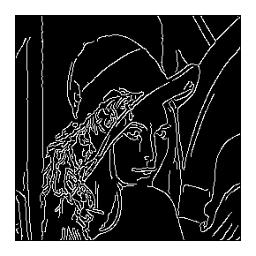
\includegraphics[width=0.25\textwidth]{./result/1_100_40}
    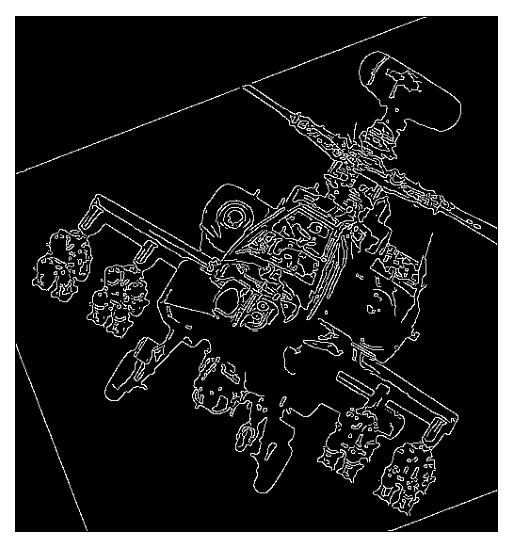
\includegraphics[width=0.25\textwidth]{./result/2_100_40}
    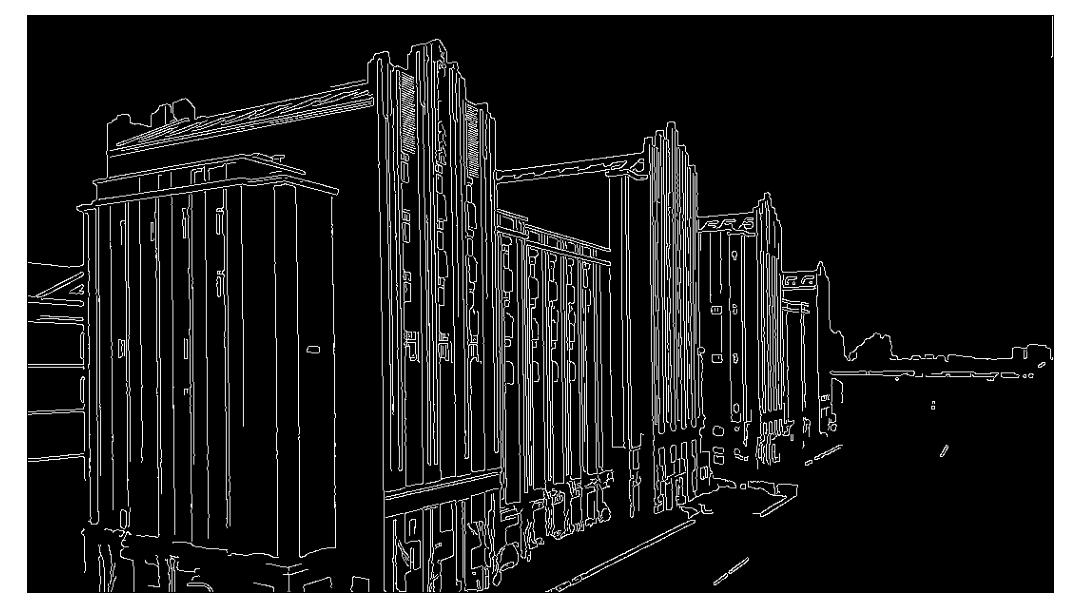
\includegraphics[width=0.25\textwidth]{./result/3_100_40}
    \caption{连接边缘结果}
\end{figure}

    可以看到,经过连接边缘处理后,图形边缘基本连接在了一起,且假边缘较少。

\subsection{不同阈值及内置函数的处理效果}

    从左至右依次为(80, 32), (100, 40), (150, 60)和内置函数(参数为(200, 80))
    代表设定的高低阈值。

\begin{figure}[h]
    \centering
    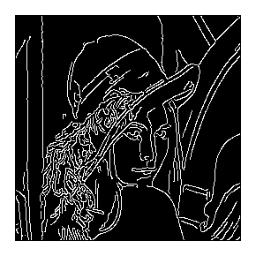
\includegraphics[width=0.22\textwidth]{./result/1_80_32}
    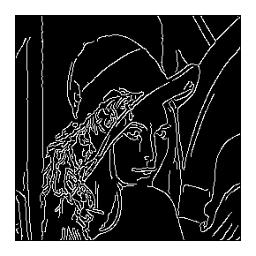
\includegraphics[width=0.22\textwidth]{./result/1_100_40}
    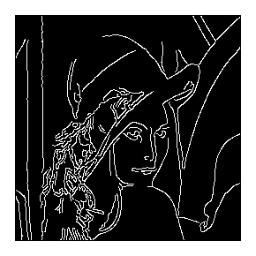
\includegraphics[width=0.22\textwidth]{./result/1_150_60}
    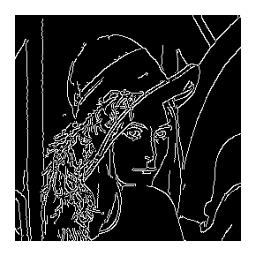
\includegraphics[width=0.22\textwidth]{./result/1_standard}
    \caption{1.jpg处理结果对比}
\end{figure}

\begin{figure}[h]
    \centering
    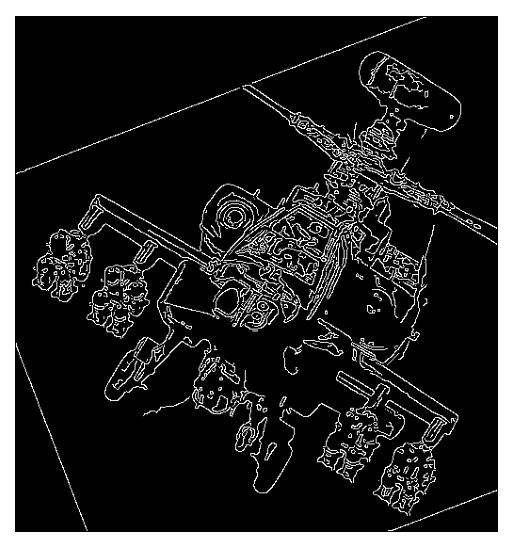
\includegraphics[width=0.22\textwidth]{./result/2_80_32}
    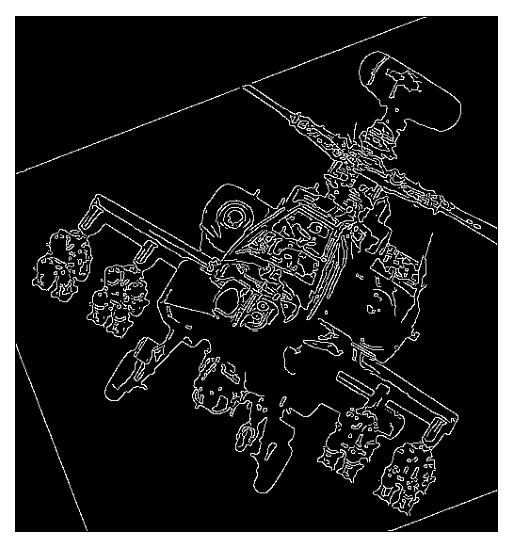
\includegraphics[width=0.22\textwidth]{./result/2_100_40}
    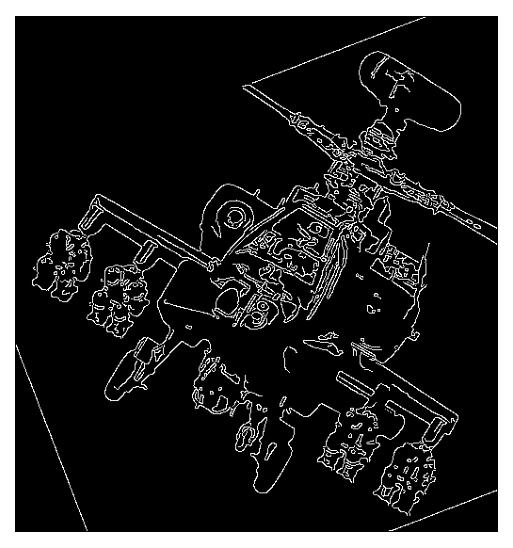
\includegraphics[width=0.22\textwidth]{./result/2_150_60}
    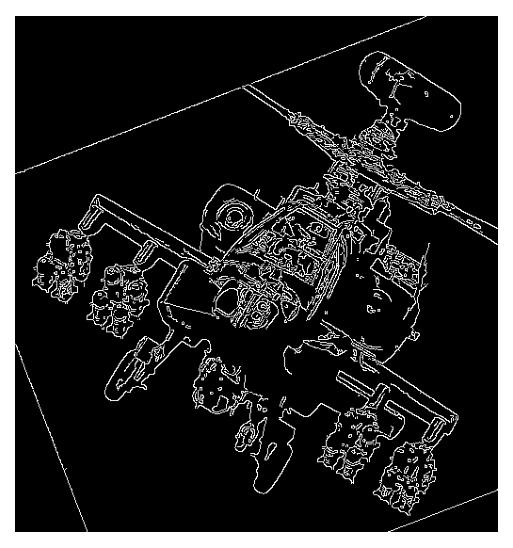
\includegraphics[width=0.22\textwidth]{./result/2_standard}
    \caption{2.jpg处理结果对比}
\end{figure}

\begin{figure}[h]
    \centering
    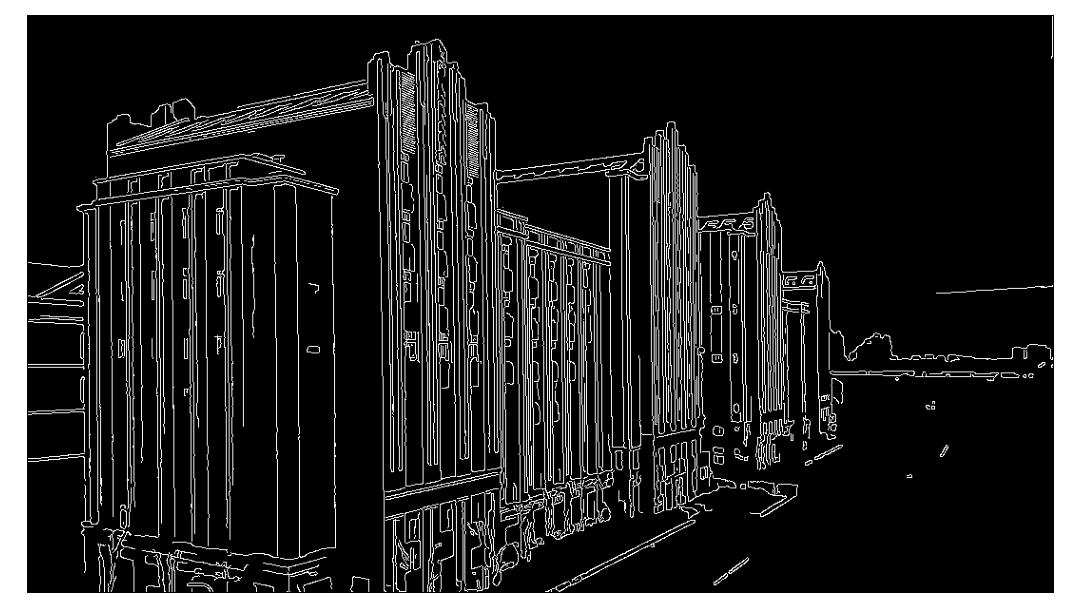
\includegraphics[width=0.22\textwidth]{./result/3_80_32}
    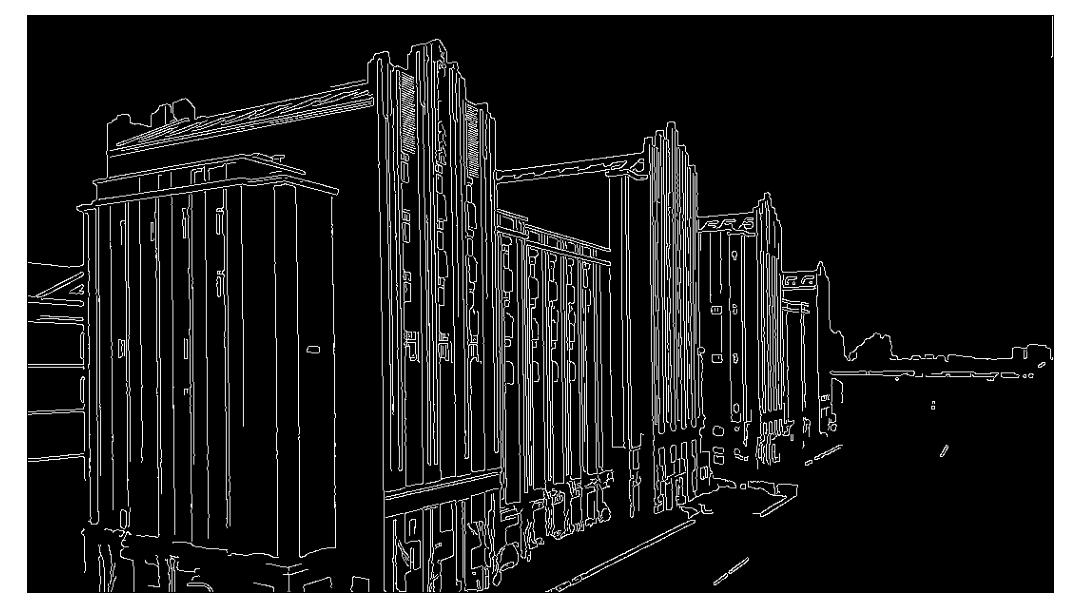
\includegraphics[width=0.22\textwidth]{./result/3_100_40}
    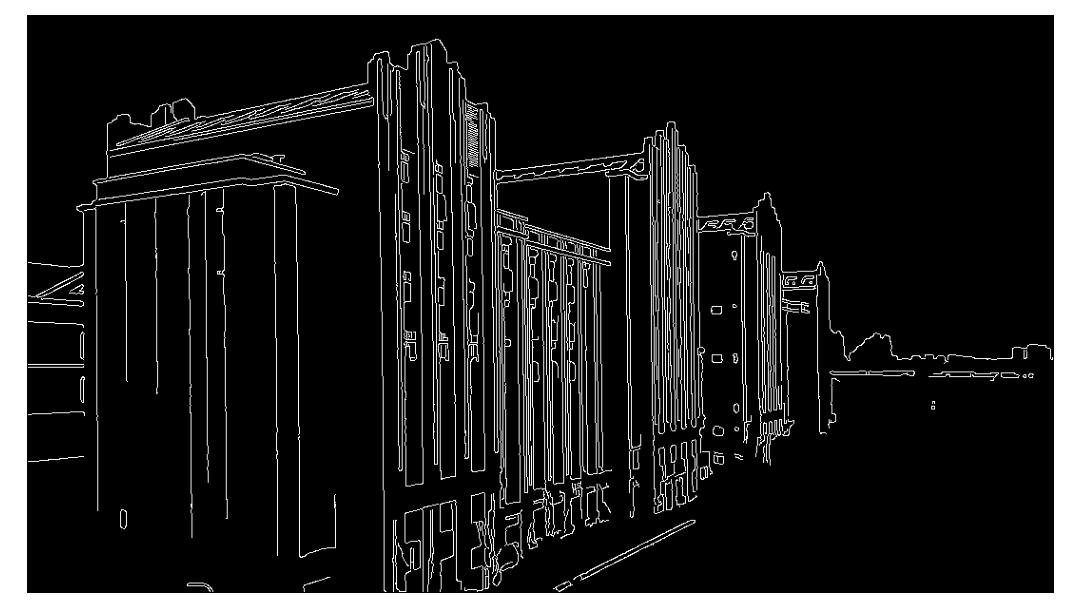
\includegraphics[width=0.22\textwidth]{./result/3_150_60}
    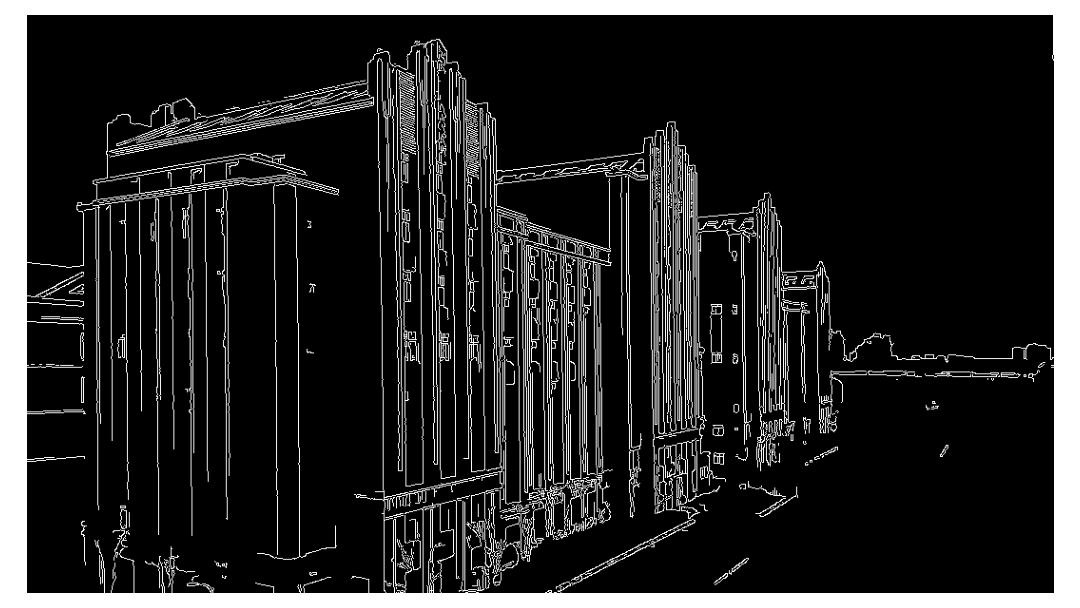
\includegraphics[width=0.22\textwidth]{./result/3_standard}
    \caption{3.jpg处理结果对比}
\end{figure}

\newpage
    结果分析:总体来看,(80,32)参数组仍存在较为明显的假边缘保留情况
    如(2.jpg组左下角的细线)
    而(150, 60)参数组虽然较好地保留了主要细节,但边缘连接情况较差,
    对于非明显梯度变化边缘(如1.jpg中的帽檐)识别情况不好。内置函数组
    可能因计算方法不完全一样,采用同样的阈值得到结果较差,因此选择单独
    设置参数,在该参数(200, 80)的情况下其特征保留的结果介于(80, 32)和
    (100, 40)组的结果之间。
    
\subsection{其他对比}
\subsubsection{不同梯度幅值算子性能比较}
    这里采用了阈值参数为(100, 40)进行控制变量,分别使用了Sobel,Prewitt
    和Canny算子(下图从左至右)。其定义见\ref{operator},为节约篇幅不再重复声明,
    且仅以1.jpg的结果作为展示(因效果差距较大),其余结果可以在name/contrast中找到。

\begin{figure}[h]
    \centering
    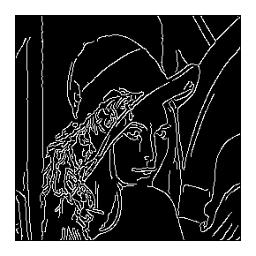
\includegraphics[width=0.25\textwidth]{./contrast/1_sobel}
    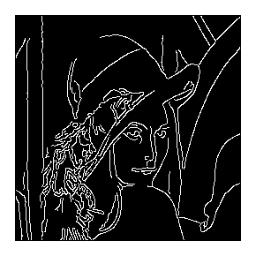
\includegraphics[width=0.25\textwidth]{./contrast/1_prewitt}
    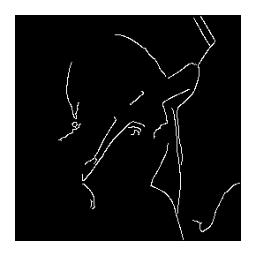
\includegraphics[width=0.25\textwidth]{./contrast/1_canny}
    \caption{使用不同算子的结果}
\end{figure}

    分析:Sobel算子较好的选取了中心特征,且由于其数值上较其他两者更大,特征更易凸显。
    相比之下Prewitt算子得到的梯度数值较小,而Canny算子更小。如进行参数调整,后
    两者效果可能会有一定提升。

\subsubsection{连接边缘定义联通数的影响}

    在边缘连接时,理想情况下我们希望得到一根细线,用于较好的刻画边缘。
    但同时我们也希望它能连接在一起,而非停止在某个端点。此时,如何定义
    边缘线联通需要引入一个参数cnt,表示该点及周围八个点中有多少点在图像
    中显示。对于一个高阈值点而言,如果cnt过小,说明该点大概率是一个端点,
    需要继续扩展;否则,认为这个点在内部,不需要继续扩展并导致边缘线变粗。

    以下就1.jpg,阈值参数为(100, 40),cnt分界值为2,3,4的结果进行展示并分析。

\begin{figure}[h]
    \centering
    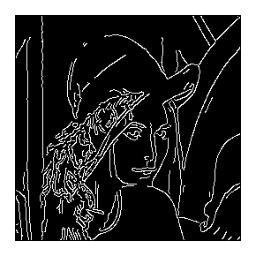
\includegraphics[width=0.25\textwidth]{./contrast/1_cnt=2}
    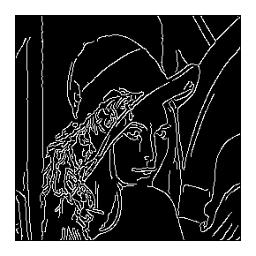
\includegraphics[width=0.25\textwidth]{./contrast/1_cnt=3}
    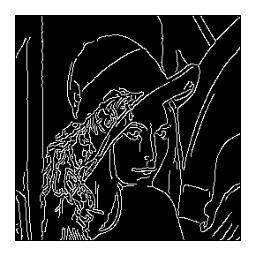
\includegraphics[width=0.25\textwidth]{./contrast/1_cnt=4}
    \caption{使用不同cnt分界值的结果}
\end{figure}

    分析:可以看到,采用cnt分界值为2得到的图连通性较差,而分界值为3和4的效果
    几乎一样。可能原因是部分分界线为斜线,如果cnt分界值为2,可能出现某端点的一侧
    及角落同时显示,此时该点被误认为是内部点而不继续扩展,导致连通性较差。

\section{实验感想}

    本次实验学习使用了Canny算法检测图形边缘,让我对边缘的认识从肉眼直观上升到了
    数学层面。多种参数的细微调整和效果比较,也让我明白需要结合实际应用灵活设置参数。
    这次学习让我对图像处理的基本概念和细节有了更深的理解,同时理解了图像处理的多
    方法、多学科结合的综合性、多样性特点。

\section{代码}
    可见name/src/edge.py
\begin{lstlisting}
import numpy as np
import cv2
import matplotlib.pyplot as plt
import math

from jedi.api.helpers import filter_follow_imports
from matplotlib import font_manager
import os
import math

font_path = 'C:\\Windows\\Fonts\\msyh.ttc' # Windows下引入微软雅黑字体
font_prop = font_manager.FontProperties(fname=font_path)

# 高斯滤波器生成
def gauss_filter(sigma=1.4, k=1):
    ax = np.arange(-k, k + 1)
    x, y = np.meshgrid(ax, ax)
    gauss_mat = np.exp(-(x ** 2 + y ** 2) / (2 * sigma ** 2))
    gauss_mat /= 2 * np.pi * sigma ** 2
    return gauss_mat / gauss_mat.sum()

# 读取灰度图像
for num in range(1, 4):
    image_grey = cv2.imread("../dataset/" + str(num) + '.jpg', cv2.IMREAD_GRAYSCALE)
    H, W = image_grey.shape
    # 高斯滤波
    gauss_core = gauss_filter()
    filter_image = cv2.filter2D(image_grey, -1, gauss_core)

    gx, gy = [], []

    # Sobel 算子计算梯度
    sx = np.array([[-1, 0, 1], [-2, 0, 2], [-1, 0, 1]])
    sy = np.array([[1, 2, 1], [0, 0, 0], [-1, -2, -1]])

    # Prewitt 算子计算梯度
    # sx = np.array([[-1, 0, 1], [-1, 0, 1], [-1, 0, 1]])
    # sy = np.array([[1, 1, 1], [0, 0, 0], [-1, -1, -1]])

    for i in range(0, H):
        gx.append([])
        gy.append([])
        for j in range(0, W):
            if i == 0 or i == H - 1 or j == 0 or j == W - 1:
                gx[-1].append(0)
                gy[-1].append(0)
                continue
            mat = filter_image[i - 1: i + 2, j - 1: j + 2]
            gx[-1].append(np.sum(mat * sx))
            gy[-1].append(np.sum(mat * sy))
    gx = np.array(gx)
    gy = np.array(gy)
    g = np.sqrt(gx ** 2 + gy ** 2)

    # Canny 算子计算梯度
    # sx = np.array([[-1, 1], [-1, 1]])
    # sy = np.array([[1, 1], [-1, -1]])
    # for i in range(H):
    #     gx.append([])
    #     gy.append([])
    #     for j in range(W):
    #         if i == 0 or i == H - 1 or j == 0 or j == W - 1:
    #             gx[-1].append(0)
    #             gy[-1].append(0)
    #             continue
    #         mat = filter_image[i : i + 2, j : j + 2]
    #         gx[-1].append(np.sum(mat * sx))
    #         gy[-1].append(np.sum(mat * sy))
    # gx = np.array(gx)
    # gy = np.array(gy)
    # g = np.sqrt(gx ** 2 + gy ** 2)

    # 非极大值抑制
    g0 = np.zeros_like(g)

    for i in range(1, H - 1):
        for j in range(1, W - 1):
            if(gx[i][j] == 0 and gy[i][j] == 0):
                continue
            if(gx[i][j] == 0 and gy[i][j] != 0):
                tmp1 = g[i - 1][j]
                tmp2 = g[i + 1][j]
                if (g[i][j] >= tmp1 and g[i][j] >= tmp2):
                    g0[i][j] = g[i][j]
                continue
            if(gx[i][j] != 0 and gy[i][j] == 0):
                tmp1 = g[i][j - 1]
                tmp2 = g[i][j + 1]
                if (g[i][j] >= tmp1 and g[i][j] >= tmp2):
                    g0[i][j] = g[i][j]
                continue
            theta = math.atan(gy[i][j] / gx[i][j]) / math.pi * 180 + 90
            tmp1, tmp2 = 0, 0
            if 0 <= theta < 45:
                k = abs(gx[i][j] / gy[i][j])
                tmp1 = g[i - 1][j] * (1 - k) + g[i - 1][j - 1] * k
                tmp2 = g[i + 1][j] * (1 - k) + g[i + 1][j + 1] * k
            if 45 <= theta < 90:
                k = abs(gy[i][j] / gx[i][j])
                tmp1 = g[i][j - 1] * (1 - k) + g[i - 1][j - 1] * k
                tmp2 = g[i][j + 1] * (1 - k) + g[i + 1][j + 1] * k
            if 90 <= theta < 135:
                k = abs(gy[i][j] / gx[i][j])
                tmp1 = g[i][j + 1] * (1 - k) + g[i - 1][j + 1] * k
                tmp2 = g[i][j - 1] * (1 - k) + g[i + 1][j - 1] * k
            if 135 <= theta < 180:
                k = abs(gx[i][j] / gy[i][j])
                tmp1 = g[i - 1][j] * (1 - k) + g[i - 1][j + 1] * k
                tmp2 = g[i + 1][j] * (1 - k) + g[i + 1][j - 1] * k
            if (g[i][j] >= tmp1 and g[i][j] >= tmp2):
                g0[i][j] = g[i][j]
    gradmap = np.zeros_like(g)
    img_bool = np.zeros_like(g)

    # 设置高低阈值
    high = 100
    low = 0.4 * high
    low = int(low)

    que = []
    for i in range(1, H - 1):
        for j in range(1, W - 1):
            if g0[i][j] >= high:
                gradmap[i][j] = high
                img_bool[i][j] = True
                que.append([i, j])
            elif g0[i][j] >= low:
                gradmap[i][j] = low

    # 边缘连接
    vis = np.zeros_like(g)
    while(len(que) != 0):
        u = que.pop(0)
        x = u[0]
        y = u[1]
        if vis[x][y]:
            continue
        img_bool[x][y] = True
        vis[x][y] = True
        cnt = 0
        for i in range(-1, 2):
            for j in range(-1, 2):
                if img_bool[x + i][y + j]:
                    cnt += 1
        if cnt <= 4:
            for i in range(-1, 2):
                for j in range(-1, 2):
                    if gradmap[x + i][y + j] >= low:
                        que.append([x + i, y + j])

    # folder_path = "../contrast"
    # os.makedirs(folder_path, exist_ok=True)
    plt.figure(figsize = (W / 100, H / 100), dpi = 100)
    plt.imshow(img_bool, cmap='gray')
    # img_canny = cv2.Canny(image_grey, 80, 200)
    # plt.imshow(img_canny, cmap='gray')
    plt.axis('off')
    # plt.tight_layout()
    # plt.savefig(folder_path + "/"+str(num)+ "_cnt=4"  + ".jpg")
    plt.show()
    plt.close()
\end{lstlisting}

\end{document}
